% Options for packages loaded elsewhere
\PassOptionsToPackage{unicode}{hyperref}
\PassOptionsToPackage{hyphens}{url}
\PassOptionsToPackage{dvipsnames,svgnames,x11names}{xcolor}
%
\documentclass[
  letterpaper,
  DIV=11,
  numbers=noendperiod]{scrartcl}

\usepackage{amsmath,amssymb}
\usepackage{iftex}
\ifPDFTeX
  \usepackage[T1]{fontenc}
  \usepackage[utf8]{inputenc}
  \usepackage{textcomp} % provide euro and other symbols
\else % if luatex or xetex
  \usepackage{unicode-math}
  \defaultfontfeatures{Scale=MatchLowercase}
  \defaultfontfeatures[\rmfamily]{Ligatures=TeX,Scale=1}
\fi
\usepackage{lmodern}
\ifPDFTeX\else  
    % xetex/luatex font selection
\fi
% Use upquote if available, for straight quotes in verbatim environments
\IfFileExists{upquote.sty}{\usepackage{upquote}}{}
\IfFileExists{microtype.sty}{% use microtype if available
  \usepackage[]{microtype}
  \UseMicrotypeSet[protrusion]{basicmath} % disable protrusion for tt fonts
}{}
\makeatletter
\@ifundefined{KOMAClassName}{% if non-KOMA class
  \IfFileExists{parskip.sty}{%
    \usepackage{parskip}
  }{% else
    \setlength{\parindent}{0pt}
    \setlength{\parskip}{6pt plus 2pt minus 1pt}}
}{% if KOMA class
  \KOMAoptions{parskip=half}}
\makeatother
\usepackage{xcolor}
\setlength{\emergencystretch}{3em} % prevent overfull lines
\setcounter{secnumdepth}{-\maxdimen} % remove section numbering
% Make \paragraph and \subparagraph free-standing
\makeatletter
\ifx\paragraph\undefined\else
  \let\oldparagraph\paragraph
  \renewcommand{\paragraph}{
    \@ifstar
      \xxxParagraphStar
      \xxxParagraphNoStar
  }
  \newcommand{\xxxParagraphStar}[1]{\oldparagraph*{#1}\mbox{}}
  \newcommand{\xxxParagraphNoStar}[1]{\oldparagraph{#1}\mbox{}}
\fi
\ifx\subparagraph\undefined\else
  \let\oldsubparagraph\subparagraph
  \renewcommand{\subparagraph}{
    \@ifstar
      \xxxSubParagraphStar
      \xxxSubParagraphNoStar
  }
  \newcommand{\xxxSubParagraphStar}[1]{\oldsubparagraph*{#1}\mbox{}}
  \newcommand{\xxxSubParagraphNoStar}[1]{\oldsubparagraph{#1}\mbox{}}
\fi
\makeatother

\usepackage{color}
\usepackage{fancyvrb}
\newcommand{\VerbBar}{|}
\newcommand{\VERB}{\Verb[commandchars=\\\{\}]}
\DefineVerbatimEnvironment{Highlighting}{Verbatim}{commandchars=\\\{\}}
% Add ',fontsize=\small' for more characters per line
\usepackage{framed}
\definecolor{shadecolor}{RGB}{241,243,245}
\newenvironment{Shaded}{\begin{snugshade}}{\end{snugshade}}
\newcommand{\AlertTok}[1]{\textcolor[rgb]{0.68,0.00,0.00}{#1}}
\newcommand{\AnnotationTok}[1]{\textcolor[rgb]{0.37,0.37,0.37}{#1}}
\newcommand{\AttributeTok}[1]{\textcolor[rgb]{0.40,0.45,0.13}{#1}}
\newcommand{\BaseNTok}[1]{\textcolor[rgb]{0.68,0.00,0.00}{#1}}
\newcommand{\BuiltInTok}[1]{\textcolor[rgb]{0.00,0.23,0.31}{#1}}
\newcommand{\CharTok}[1]{\textcolor[rgb]{0.13,0.47,0.30}{#1}}
\newcommand{\CommentTok}[1]{\textcolor[rgb]{0.37,0.37,0.37}{#1}}
\newcommand{\CommentVarTok}[1]{\textcolor[rgb]{0.37,0.37,0.37}{\textit{#1}}}
\newcommand{\ConstantTok}[1]{\textcolor[rgb]{0.56,0.35,0.01}{#1}}
\newcommand{\ControlFlowTok}[1]{\textcolor[rgb]{0.00,0.23,0.31}{\textbf{#1}}}
\newcommand{\DataTypeTok}[1]{\textcolor[rgb]{0.68,0.00,0.00}{#1}}
\newcommand{\DecValTok}[1]{\textcolor[rgb]{0.68,0.00,0.00}{#1}}
\newcommand{\DocumentationTok}[1]{\textcolor[rgb]{0.37,0.37,0.37}{\textit{#1}}}
\newcommand{\ErrorTok}[1]{\textcolor[rgb]{0.68,0.00,0.00}{#1}}
\newcommand{\ExtensionTok}[1]{\textcolor[rgb]{0.00,0.23,0.31}{#1}}
\newcommand{\FloatTok}[1]{\textcolor[rgb]{0.68,0.00,0.00}{#1}}
\newcommand{\FunctionTok}[1]{\textcolor[rgb]{0.28,0.35,0.67}{#1}}
\newcommand{\ImportTok}[1]{\textcolor[rgb]{0.00,0.46,0.62}{#1}}
\newcommand{\InformationTok}[1]{\textcolor[rgb]{0.37,0.37,0.37}{#1}}
\newcommand{\KeywordTok}[1]{\textcolor[rgb]{0.00,0.23,0.31}{\textbf{#1}}}
\newcommand{\NormalTok}[1]{\textcolor[rgb]{0.00,0.23,0.31}{#1}}
\newcommand{\OperatorTok}[1]{\textcolor[rgb]{0.37,0.37,0.37}{#1}}
\newcommand{\OtherTok}[1]{\textcolor[rgb]{0.00,0.23,0.31}{#1}}
\newcommand{\PreprocessorTok}[1]{\textcolor[rgb]{0.68,0.00,0.00}{#1}}
\newcommand{\RegionMarkerTok}[1]{\textcolor[rgb]{0.00,0.23,0.31}{#1}}
\newcommand{\SpecialCharTok}[1]{\textcolor[rgb]{0.37,0.37,0.37}{#1}}
\newcommand{\SpecialStringTok}[1]{\textcolor[rgb]{0.13,0.47,0.30}{#1}}
\newcommand{\StringTok}[1]{\textcolor[rgb]{0.13,0.47,0.30}{#1}}
\newcommand{\VariableTok}[1]{\textcolor[rgb]{0.07,0.07,0.07}{#1}}
\newcommand{\VerbatimStringTok}[1]{\textcolor[rgb]{0.13,0.47,0.30}{#1}}
\newcommand{\WarningTok}[1]{\textcolor[rgb]{0.37,0.37,0.37}{\textit{#1}}}

\providecommand{\tightlist}{%
  \setlength{\itemsep}{0pt}\setlength{\parskip}{0pt}}\usepackage{longtable,booktabs,array}
\usepackage{calc} % for calculating minipage widths
% Correct order of tables after \paragraph or \subparagraph
\usepackage{etoolbox}
\makeatletter
\patchcmd\longtable{\par}{\if@noskipsec\mbox{}\fi\par}{}{}
\makeatother
% Allow footnotes in longtable head/foot
\IfFileExists{footnotehyper.sty}{\usepackage{footnotehyper}}{\usepackage{footnote}}
\makesavenoteenv{longtable}
\usepackage{graphicx}
\makeatletter
\def\maxwidth{\ifdim\Gin@nat@width>\linewidth\linewidth\else\Gin@nat@width\fi}
\def\maxheight{\ifdim\Gin@nat@height>\textheight\textheight\else\Gin@nat@height\fi}
\makeatother
% Scale images if necessary, so that they will not overflow the page
% margins by default, and it is still possible to overwrite the defaults
% using explicit options in \includegraphics[width, height, ...]{}
\setkeys{Gin}{width=\maxwidth,height=\maxheight,keepaspectratio}
% Set default figure placement to htbp
\makeatletter
\def\fps@figure{htbp}
\makeatother

\KOMAoption{captions}{tableheading}
\makeatletter
\@ifpackageloaded{caption}{}{\usepackage{caption}}
\AtBeginDocument{%
\ifdefined\contentsname
  \renewcommand*\contentsname{Table of contents}
\else
  \newcommand\contentsname{Table of contents}
\fi
\ifdefined\listfigurename
  \renewcommand*\listfigurename{List of Figures}
\else
  \newcommand\listfigurename{List of Figures}
\fi
\ifdefined\listtablename
  \renewcommand*\listtablename{List of Tables}
\else
  \newcommand\listtablename{List of Tables}
\fi
\ifdefined\figurename
  \renewcommand*\figurename{Figure}
\else
  \newcommand\figurename{Figure}
\fi
\ifdefined\tablename
  \renewcommand*\tablename{Table}
\else
  \newcommand\tablename{Table}
\fi
}
\@ifpackageloaded{float}{}{\usepackage{float}}
\floatstyle{ruled}
\@ifundefined{c@chapter}{\newfloat{codelisting}{h}{lop}}{\newfloat{codelisting}{h}{lop}[chapter]}
\floatname{codelisting}{Listing}
\newcommand*\listoflistings{\listof{codelisting}{List of Listings}}
\makeatother
\makeatletter
\makeatother
\makeatletter
\@ifpackageloaded{caption}{}{\usepackage{caption}}
\@ifpackageloaded{subcaption}{}{\usepackage{subcaption}}
\makeatother

\ifLuaTeX
  \usepackage{selnolig}  % disable illegal ligatures
\fi
\usepackage{bookmark}

\IfFileExists{xurl.sty}{\usepackage{xurl}}{} % add URL line breaks if available
\urlstyle{same} % disable monospaced font for URLs
\hypersetup{
  pdftitle={QTM 350 Final Project -- School Enrollment Trends Analysis},
  pdfauthor={Da Eun Kim (2483332); Alix Morales (2594298); Katie Park (2563640); Yoonsuh Park (2499926)},
  colorlinks=true,
  linkcolor={blue},
  filecolor={Maroon},
  citecolor={Blue},
  urlcolor={Blue},
  pdfcreator={LaTeX via pandoc}}


\title{QTM 350 Final Project -- School Enrollment Trends Analysis}
\author{Da Eun Kim (2483332) \and Alix Morales (2594298) \and Katie Park
(2563640) \and Yoonsuh Park (2499926)}
\date{2024-12-09}

\begin{document}
\maketitle

\renewcommand*\contentsname{Table of contents}
{
\hypersetup{linkcolor=}
\setcounter{tocdepth}{2}
\tableofcontents
}

\section{Introduction}\label{introduction}

Education is a cornerstone of sustainable development, playing a pivotal
role in shaping economic and social outcomes. School enrollment rates,
which measure access to education at primary, secondary, and tertiary
levels, serve as critical indicators of a country's progress toward
achieving universal education. This project explores global patterns and
disparities in school enrollment using data from the World Bank's World
Development Indicators (WDI) database. By examining trends over time,
identifying leading and lagging countries, and analyzing regional
differences, this study sheds light on the successes and persistent
challenges in global education systems.

Focusing on three key indicators---primary enrollment (\% gross),
secondary enrollment (\% gross), and tertiary enrollment (\%
gross)---this analysis investigates the relationships between education
levels and their evolution over time. Additionally, it evaluates how
regions and countries vary in their educational performance,
highlighting areas for policy intervention. This study aims to provide
actionable insights into the state of global education, contributing to
the broader discourse on achieving equitable and inclusive access to
quality education worldwide.

\section{Data Description}\label{data-description}

This dataset is a long-format representation of World Development
Indicators (WDI), capturing socio-economic and developmental statistics
across multiple countries and regions. It includes 664 entries spanning
a range of indicators, such as school enrollment rates at different
educational levels. The data consists of seven columns:
\texttt{country\_name}, \texttt{country\_code}, \texttt{series\_name}
(indicator name), \texttt{series\_code} (indicator code), \texttt{year},
\texttt{value} (observed statistic), and \texttt{region} (geographical
classification). Each row corresponds to a specific indicator for a
country in a given year, making it suitable for time-series analysis and
cross-country comparisons. The dataset provides insights into regional
and global trends, supporting research on education, economic
development, and social progress.

Primary Enrollment (\% gross): Indicator code SE.PRM.ENRR. Secondary
Enrollment (\% gross): Indicator code SE.SEC.ENRR. Tertiary Enrollment
(\% gross): Indicator code SE.TER.ENRR. Countries and Regions: Data is
available for countries worldwide, categorized into regions such as
``South Asia,'' ``Sub-Saharan Africa,'' etc. Years: The dataset includes
time-series data, enabling the analysis of enrollment trends over time.
Variables: The dataset contains numerical values for enrollment rates
(value) along with metadata such as country name, region, and year. The
dataset has been cleaned for consistency: no missing values were
observed in key columns, and all columns have appropriate data types.

\section{Data Analysis}\label{data-analysis}

\begin{Shaded}
\begin{Highlighting}[]
\ImportTok{import}\NormalTok{ pandas }\ImportTok{as}\NormalTok{ pd}
\NormalTok{wdi\_data }\OperatorTok{=}\NormalTok{ pd.read\_csv(}\StringTok{"wdi\_data\_long.csv"}\NormalTok{)}
\end{Highlighting}
\end{Shaded}

\subsection{Global Trends in School Enrollment Over
Time}\label{global-trends-in-school-enrollment-over-time}

This analysis examines the global trends in gross enrollment rates
across primary, secondary, and tertiary education levels over time. By
grouping data by year and indicator, we calculate global averages and
plot these trends.

\begin{Shaded}
\begin{Highlighting}[]
\CommentTok{\#1. Global Trends in School Enrollment Over Time}
\ImportTok{import}\NormalTok{ matplotlib.pyplot }\ImportTok{as}\NormalTok{ plt}

\CommentTok{\# Extract relevant indicators for analysis}

\NormalTok{relevant\_indicators }\OperatorTok{=}\NormalTok{ [}\StringTok{\textquotesingle{}SE.PRM.ENRR\textquotesingle{}}\NormalTok{, }\StringTok{\textquotesingle{}SE.SEC.ENRR\textquotesingle{}}\NormalTok{, }\StringTok{\textquotesingle{}SE.TER.ENRR\textquotesingle{}}\NormalTok{]}

\NormalTok{filtered\_data }\OperatorTok{=}\NormalTok{ wdi\_data[wdi\_data[}\StringTok{\textquotesingle{}series\_code\textquotesingle{}}\NormalTok{].isin(relevant\_indicators)]}

\CommentTok{\# Group by year and calculate global averages for each indicator}

\NormalTok{trend\_data }\OperatorTok{=}\NormalTok{ filtered\_data.groupby([}\StringTok{\textquotesingle{}year\textquotesingle{}}\NormalTok{, }\StringTok{\textquotesingle{}series\_name\textquotesingle{}}\NormalTok{])[}\StringTok{\textquotesingle{}value\textquotesingle{}}\NormalTok{].mean().reset\_index()}

\CommentTok{\# Plot trends over time}

\NormalTok{plt.figure(figsize}\OperatorTok{=}\NormalTok{(}\DecValTok{12}\NormalTok{, }\DecValTok{6}\NormalTok{))}

\ControlFlowTok{for}\NormalTok{ indicator }\KeywordTok{in}\NormalTok{ trend\_data[}\StringTok{\textquotesingle{}series\_name\textquotesingle{}}\NormalTok{].unique():}
\NormalTok{    indicator\_data }\OperatorTok{=}\NormalTok{ trend\_data[trend\_data[}\StringTok{\textquotesingle{}series\_name\textquotesingle{}}\NormalTok{] }\OperatorTok{==}\NormalTok{ indicator]}
\NormalTok{    plt.plot(indicator\_data[}\StringTok{\textquotesingle{}year\textquotesingle{}}\NormalTok{], indicator\_data[}\StringTok{\textquotesingle{}value\textquotesingle{}}\NormalTok{], label}\OperatorTok{=}\NormalTok{indicator)}

\NormalTok{plt.title(}\StringTok{\textquotesingle{}Global Trends in School Enrollment Over Time\textquotesingle{}}\NormalTok{, fontsize}\OperatorTok{=}\DecValTok{14}\NormalTok{)}
\NormalTok{plt.xlabel(}\StringTok{\textquotesingle{}Year\textquotesingle{}}\NormalTok{, fontsize}\OperatorTok{=}\DecValTok{12}\NormalTok{)}
\NormalTok{plt.ylabel(}\StringTok{\textquotesingle{}Enrollment Rate (}\SpecialCharTok{\% g}\StringTok{ross)\textquotesingle{}}\NormalTok{, fontsize}\OperatorTok{=}\DecValTok{12}\NormalTok{)}
\NormalTok{plt.legend(title}\OperatorTok{=}\StringTok{\textquotesingle{}Education Level\textquotesingle{}}\NormalTok{)}
\NormalTok{plt.grid(}\VariableTok{True}\NormalTok{)}
\NormalTok{plt.show()}
\end{Highlighting}
\end{Shaded}

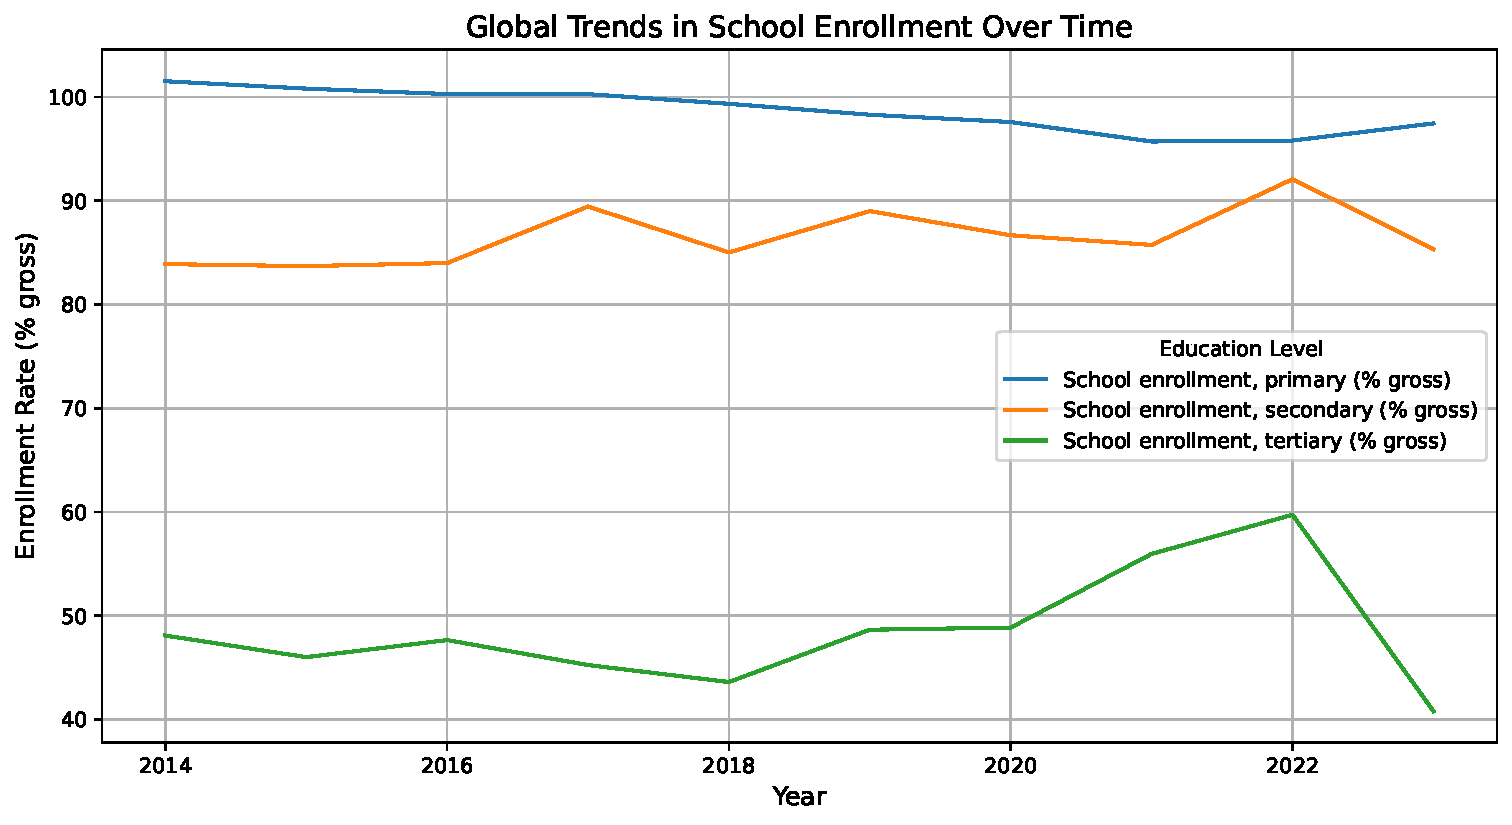
\includegraphics{report_files/figure-pdf/cell-3-output-1.pdf}

\emph{Figure 1: Trends in global school enrollment rates over time,
showing gross enrollment rates for primary, secondary, and tertiary
education. Primary enrollment rates are consistently high, while
secondary and tertiary levels show gradual increases, reflecting
progress in global education access.}

\subsection{Regional Comparison of Mean Enrollment Rates by
Indicator}\label{regional-comparison-of-mean-enrollment-rates-by-indicator}

This analysis compares average enrollment rates by education level
(primary, secondary, tertiary) across different regions. By calculating
mean rates per region, the bar chart highlights disparities in education
access.

\begin{Shaded}
\begin{Highlighting}[]
\CommentTok{\#2. Regional Comparison of Mean Enrollment Rates by Indicator}

\NormalTok{indicator\_region\_averages }\OperatorTok{=}\NormalTok{ wdi\_data.groupby([}\StringTok{\textquotesingle{}series\_name\textquotesingle{}}\NormalTok{, }\StringTok{\textquotesingle{}region\textquotesingle{}}\NormalTok{])[}\StringTok{\textquotesingle{}value\textquotesingle{}}\NormalTok{].mean().unstack()}
\NormalTok{indicator\_region\_averages.plot(kind}\OperatorTok{=}\StringTok{\textquotesingle{}bar\textquotesingle{}}\NormalTok{, figsize}\OperatorTok{=}\NormalTok{(}\DecValTok{12}\NormalTok{, }\DecValTok{8}\NormalTok{))}
\NormalTok{plt.title(}\StringTok{"Average Enrollment Rates by Indicator and Region"}\NormalTok{, fontsize}\OperatorTok{=}\DecValTok{14}\NormalTok{)}
\NormalTok{plt.xlabel(}\StringTok{"Education Indicator"}\NormalTok{, fontsize}\OperatorTok{=}\DecValTok{12}\NormalTok{)}
\NormalTok{plt.ylabel(}\StringTok{"Mean Enrollment Rate (\%)"}\NormalTok{, fontsize}\OperatorTok{=}\DecValTok{12}\NormalTok{)}
\NormalTok{plt.xticks(rotation}\OperatorTok{=}\DecValTok{45}\NormalTok{, ha}\OperatorTok{=}\StringTok{\textquotesingle{}right\textquotesingle{}}\NormalTok{)}
\NormalTok{plt.legend(title}\OperatorTok{=}\StringTok{\textquotesingle{}Region\textquotesingle{}}\NormalTok{, bbox\_to\_anchor}\OperatorTok{=}\NormalTok{(}\FloatTok{1.05}\NormalTok{, }\DecValTok{1}\NormalTok{), loc}\OperatorTok{=}\StringTok{\textquotesingle{}upper left\textquotesingle{}}\NormalTok{)}
\NormalTok{plt.tight\_layout()}
\NormalTok{plt.show()}
\end{Highlighting}
\end{Shaded}

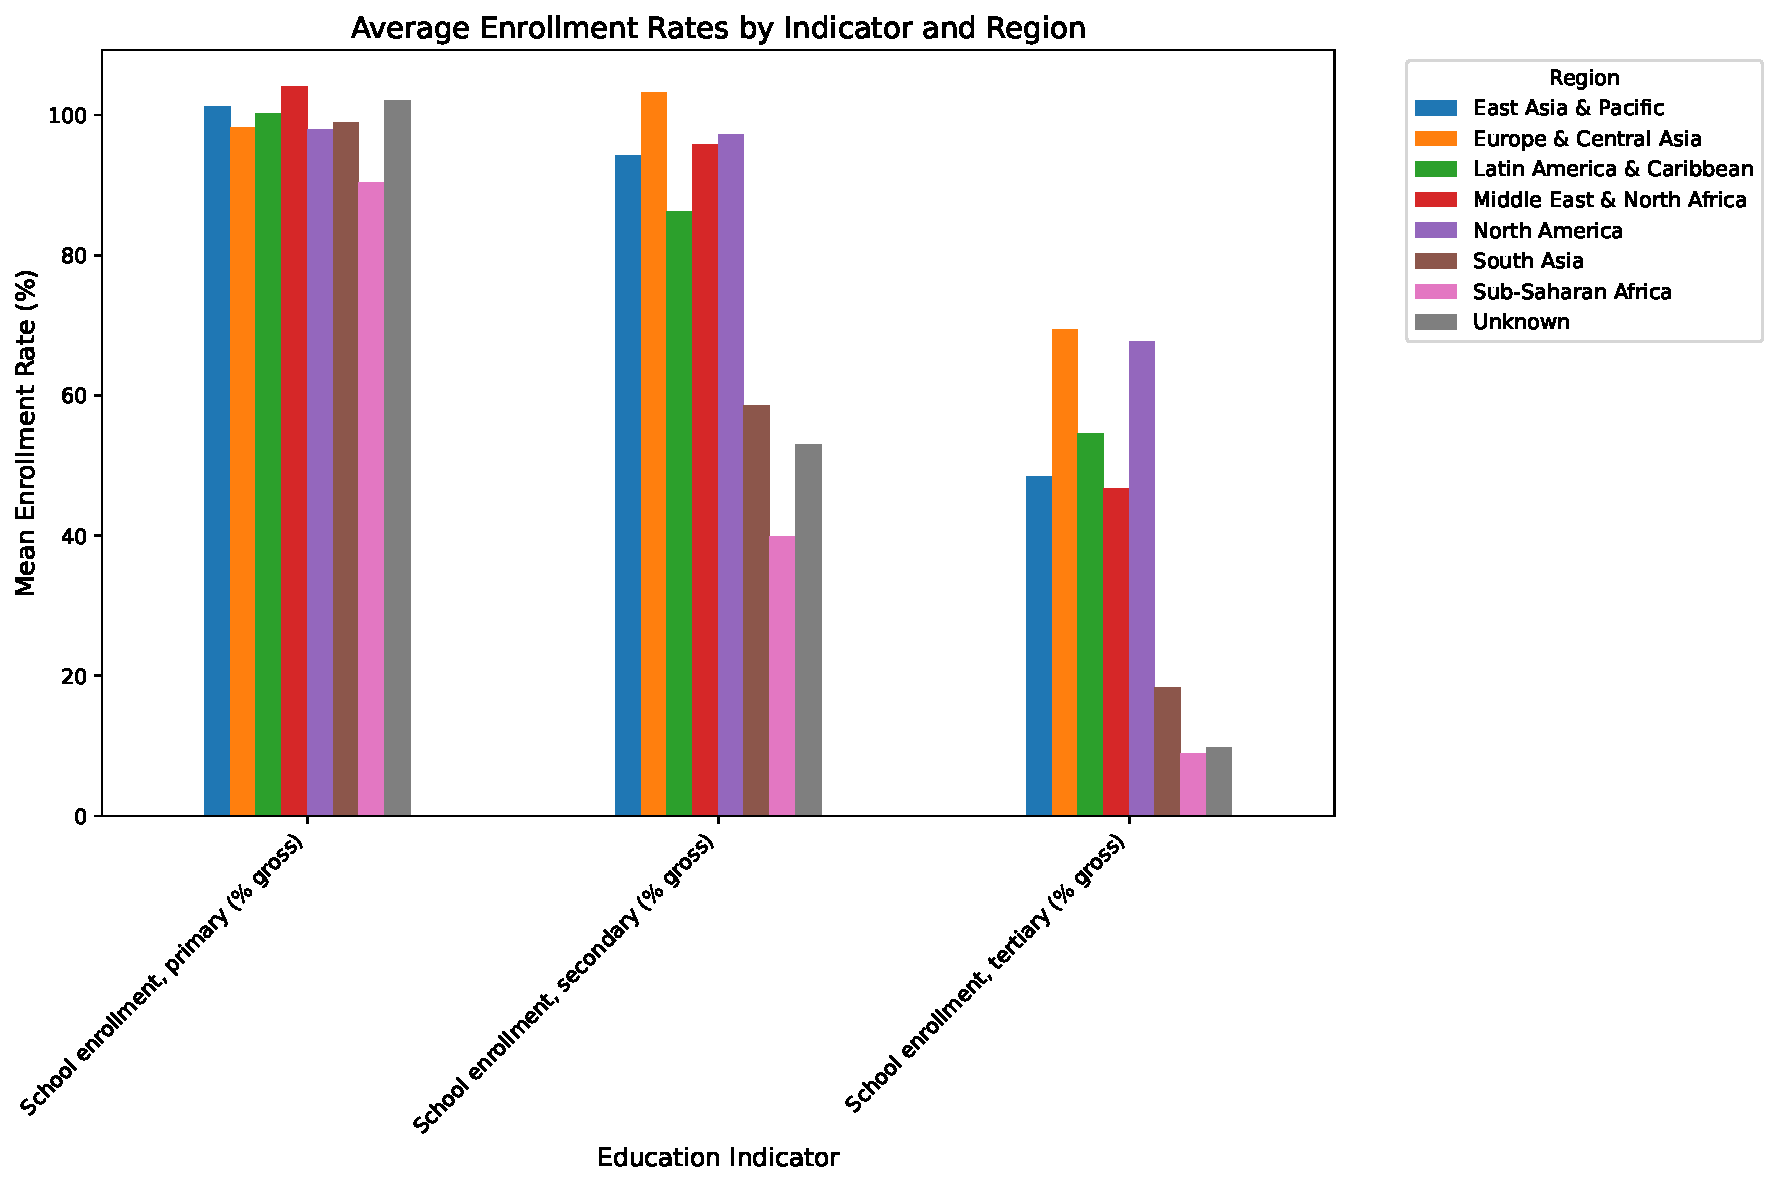
\includegraphics{report_files/figure-pdf/cell-4-output-1.pdf}

\emph{Figure 2: Average school enrollment rates by region and education
level, illustrating significant disparities. Developed regions exhibit
higher enrollment rates across all levels, while Sub-Saharan Africa and
South Asia lag behind, especially in tertiary education.}

\subsection{Correlation Between Primary, Secondary, and Tertiary
Enrollment}\label{correlation-between-primary-secondary-and-tertiary-enrollment}

This analysis explores the relationship between enrollment rates at
primary, secondary, and tertiary levels. A heatmap visualizes Pearson
correlation coefficients.

\begin{Shaded}
\begin{Highlighting}[]
\CommentTok{\#3. Correlation Between Primary, Secondary and Tertiary Indictors}

\CommentTok{\# Filter data to include only relevant indicators}
\NormalTok{filtered\_data }\OperatorTok{=}\NormalTok{ wdi\_data[wdi\_data[}\StringTok{\textquotesingle{}series\_name\textquotesingle{}}\NormalTok{].isin([}
    \StringTok{\textquotesingle{}School enrollment, primary (}\SpecialCharTok{\% g}\StringTok{ross)\textquotesingle{}}\NormalTok{,}
    \StringTok{\textquotesingle{}School enrollment, secondary (}\SpecialCharTok{\% g}\StringTok{ross)\textquotesingle{}}\NormalTok{,}
    \StringTok{\textquotesingle{}School enrollment, tertiary (}\SpecialCharTok{\% g}\StringTok{ross)\textquotesingle{}}
\NormalTok{])]}

\CommentTok{\# Pivot data to have indicators as columns}
\NormalTok{pivoted\_data }\OperatorTok{=}\NormalTok{ filtered\_data.pivot\_table(}
\NormalTok{    index}\OperatorTok{=}\NormalTok{[}\StringTok{\textquotesingle{}country\_name\textquotesingle{}}\NormalTok{, }\StringTok{\textquotesingle{}year\textquotesingle{}}\NormalTok{], }
\NormalTok{    columns}\OperatorTok{=}\StringTok{\textquotesingle{}series\_name\textquotesingle{}}\NormalTok{, }
\NormalTok{    values}\OperatorTok{=}\StringTok{\textquotesingle{}value\textquotesingle{}}
\NormalTok{).dropna()}

\CommentTok{\# Rename columns for easier reference}
\NormalTok{pivoted\_data.columns }\OperatorTok{=}\NormalTok{ [}\StringTok{\textquotesingle{}Primary Enrollment\textquotesingle{}}\NormalTok{, }\StringTok{\textquotesingle{}Secondary Enrollment\textquotesingle{}}\NormalTok{, }\StringTok{\textquotesingle{}Tertiary Enrollment\textquotesingle{}}\NormalTok{]}

\CommentTok{\# Calculate Pearson correlation coefficients}
\NormalTok{correlation\_matrix }\OperatorTok{=}\NormalTok{ pivoted\_data.corr()}

\ImportTok{import}\NormalTok{ seaborn }\ImportTok{as}\NormalTok{ sns}

\CommentTok{\# Plotting the correlation heatmap}
\NormalTok{plt.figure(figsize}\OperatorTok{=}\NormalTok{(}\DecValTok{8}\NormalTok{, }\DecValTok{6}\NormalTok{))}
\NormalTok{sns.heatmap(correlation\_matrix, annot}\OperatorTok{=}\VariableTok{True}\NormalTok{, fmt}\OperatorTok{=}\StringTok{".2f"}\NormalTok{, cmap}\OperatorTok{=}\StringTok{"coolwarm"}\NormalTok{, cbar}\OperatorTok{=}\VariableTok{True}\NormalTok{)}
\NormalTok{plt.title(}\StringTok{"Correlation Heatmap: Primary, Secondary, and Tertiary Enrollment"}\NormalTok{)}
\NormalTok{plt.show()}
\end{Highlighting}
\end{Shaded}

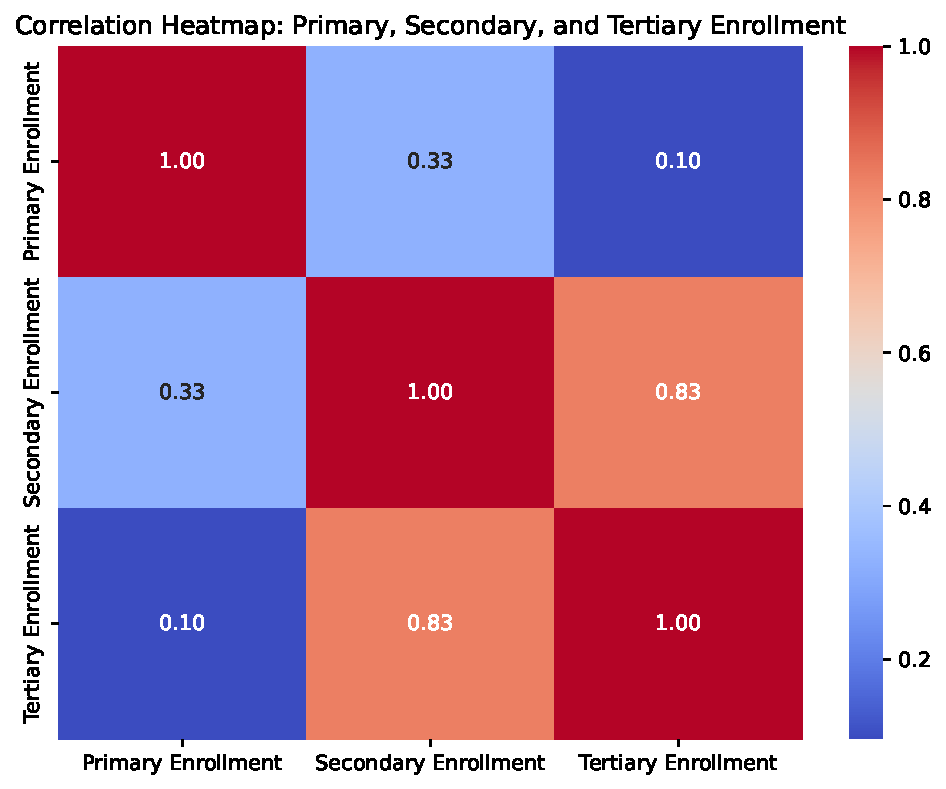
\includegraphics{report_files/figure-pdf/cell-5-output-1.pdf}

\emph{Figure 3: Correlation heatmap of primary, secondary, and tertiary
school enrollment rates. The strong correlations indicate a cascading
effect, where higher primary enrollment positively influences subsequent
levels of education.}

\section{Results and Discussion}\label{results-and-discussion}

\subsection{Global Trends in School Enrollment Over
Time}\label{global-trends-in-school-enrollment-over-time-1}

\begin{itemize}
\tightlist
\item
  Primary Enrollment: Typically the highest across all years, reflecting
  widespread prioritization of basic education globally.
\item
  Secondary Enrollment: Generally lower than primary but shows an upward
  trend, indicating improvements in access to education beyond primary
  school.
\item
  Tertiary Enrollment: The lowest but with significant growth over the
  years, suggesting increasing opportunities for higher education
  globally.
\end{itemize}

These trends highlight global efforts to enhance education access, with
significant progress at all levels, particularly in tertiary education.

\subsection{Regional Comparison of Mean Enrollment Rates by
Indicator}\label{regional-comparison-of-mean-enrollment-rates-by-indicator-1}

\begin{itemize}
\tightlist
\item
  Developed Regions: Tend to have high enrollment rates across all
  levels, indicating well-established education systems.
\item
  Developing Regions: Display gaps, especially in secondary and tertiary
  levels, pointing to challenges like economic barriers and lack of
  infrastructure.
\item
  Notable Gaps: Sub-Saharan Africa and South Asia show significantly
  lower tertiary enrollment rates, emphasizing regional inequalities.
\end{itemize}

Such comparisons underline the need for targeted policies to address
disparities and improve access in underperforming regions.

\subsection{Correlation Between Primary, Secondary, and Tertiary
Enrollment}\label{correlation-between-primary-secondary-and-tertiary-enrollment-1}

\begin{itemize}
\tightlist
\item
  Primary vs.~Secondary: Strong positive correlation, reflecting that
  countries with high primary enrollment are likely to achieve better
  secondary enrollment.
\item
  Secondary vs.~Tertiary: Moderate to strong correlation, highlighting
  that success at secondary education often translates into higher
  tertiary participation.
\item
  Primary vs.~Tertiary: Weak to moderate correlation, suggesting that
  barriers between these levels may be distinct.
\end{itemize}

These findings emphasize the interconnectedness of educational levels,
where improvements in one level positively influence others, though with
diminishing returns as the education level increases. \hspace{0pt}

\section{Conclusion}\label{conclusion}

In conclusion, the analysis of global school enrollment trends provides
valuable insights into the progress and challenges in achieving
universal education. Primary education exhibits consistently high
enrollment rates, reflecting global commitments to foundational
education access. However, the disparities in secondary and tertiary
enrollment highlight persistent inequalities, particularly in developing
regions such as Sub-Saharan Africa and South Asia. These disparities
emphasize the need for targeted policy interventions, such as improving
education infrastructure, addressing economic barriers, and enhancing
teacher training.

Moreover, the positive correlation between primary, secondary, and
tertiary enrollment underscores the interconnected nature of education
levels. Policies promoting smooth transitions between these stages are
essential for long-term educational success. The upward trend in
tertiary enrollment is promising, indicating growing opportunities for
higher education. However, achieving equitable access remains a
challenge, requiring sustained efforts from governments, international
organizations, and communities.

By shedding light on these patterns, this study underscores the
importance of data-driven approaches to education policymaking. Future
research could expand on this analysis by exploring the impact of
socioeconomic factors, gender disparities, and digital access on
enrollment trends, offering a more holistic view of global education
systems.




\end{document}
